\chapter{等式松弛机制}\label{chap:method2}

本章节主要介绍局部搜索算法在LS\_NRA处理等式约束时的松弛技术,主要可以分为两个阶段:松弛阶段和恢复阶段。
首先,本章节考虑到局部搜索迭代算法的效率问题,引入赋值复杂度的概念,并提出非线性实数理论独有的无理数赋值挑战。
紧接着,本文提出一种等式松弛方法来暂时扩大约束的可行域,从而保证了有理数赋值,使得算法可以找到附近的近似解。
然后,本文探讨了算法最后的恢复阶段,即近似解如何恢复为原问题的精确解,并提出了具体的懒惰版本的实现方法。
最后,本文介绍了其他的一些可行的改进策略。

\section{代数数赋值的复杂度}
在SMT问题的四种主流算术理论(线性整数理论、线性实数理论、非线性整数理论、非线性实数理论)中,非线性实数理论(NRA)因为其存在高次多项式约束与潜在的无理数赋值问题而最难处理。这些情况基本发生在等式约束上,例如$x^2 + y^2 = 2$等。对于局部搜索迭代而言,尽管在计算机中可以使用代数数表示无理数,但无理数赋值问题带来的仍是多项式评估的效率低下,进而影响到实根隔离与计算可行域等操作。除此之外,一些分母较大的代数数仍然会影响计算速度。

在参考文献\cite{multilinear,LiXZ23}中,以往的工作都尽量避免了代数数引发的计算问题,因此将非线性问题限定为多线性约束(multilinear)或至少包含一个线性项的等式约束上。其中,工作\cite{multilinear}考虑了有理数赋值的分母大小问题,并将其作为操作得分相同时的打破平均策略。

我们的工作考虑了非线性实数的全部测试样例,一个关键的优化是尽量减少复杂赋值的出现频率。为此,我们首先定义赋值之间的复杂度关系如下:

\begin{definition}{\textbf{赋值复杂度(Complexity of values)}}
\label{def:complexity}
我们定义代数数上的偏序$\prec_c$如下。$x \prec_c y$当且仅当以下任何一种情况成立:

\begin{itemize}
    \item $x$和$y$都是有理数,且$x$的分母小于$y$的分母。
    \item $x$是有理数,而$y$是无理数。
\end{itemize}
当$x \prec_c y$或者$y \prec_c x$均不成立时,我们认为$x$和$y$的复杂度相当,记为$x \sim_c y$。
\end{definition}

\section{松弛机制}
我们将等式的松弛机制简单描述如下:每次当等式或者不等式约束迫使某一个变量必须赋值为一个相对复杂的代数数时,我们会暂时松弛这些约束,使用复杂度相对低的松弛解,然后以松弛的形式继续局部搜索的迭代过程。在具体实现上,我们引入以下两个参数来设置算法门槛:
\begin{itemize}
    \item $\epsilon_v$:根据定义\ref{def:complexity}衡量表示代数数复杂度,取值为$10^{-4}$。
    \item $\epsilon_p$:多项式约束松弛的程度,见定义\ref{def:relaxation},取值为$10^{-4}$。
\end{itemize}


需要注意的是,在非线性实数理论中,无理数赋值并不完全由等式约束所要求,可能是多个形如$p \ge 0$或$p \le 0$的约束交集所决定。因此,本文实际上讨论的是严格多项式的松弛问题。具体的松弛机制定义如下:

\begin{definition}{\textbf{约束松弛(Relaxation of constraints)}}
\label{def:relaxation}
\begin{itemize}
    \item 如果约束形如$p = 0$,将其松弛为$p < \epsilon_p$和$p > -\epsilon_p$。
    \item 如果约束形如$p \ge 0$,将其松弛为$p > -\epsilon_p$。同样的,如果约束形如$p \le 0$,将其松弛为$p < \epsilon_p$。
\end{itemize}
\end{definition}

在局部搜索迭代中,当我们计算某个变量$v$的分数时,如果最优的分数来自于一个点区间,我们会记录这个点区间对应的边界子句标号。如果变量$v$在后续的迭代中被选中,并且其赋值比之前的赋值和$\epsilon_v$的复杂度高,那么记录的等式约束和严格不等式约束都会被松弛。也就是说,我们的松弛机制是懒惰的,只有当无理数赋值十分必要时才会进行,而非直接在预处理阶段进行。当松弛之后,局部搜索算法继续迭代,并且文字和多项式的评估完全按照松弛后的形式进行。


\section{恢复机制}
当局部搜索算法找到了一个松弛形式下的“可行解”之后,这个解被称为\textbf{近似解}。事实上,这并不能确保精确解的存在,鉴于SMT问题的要求,我们仍然需要找到原始状态下的附近精确解。本工作主要尝试两种方法。

第一种方法是对于松弛状态下的约束进行启发式分析,尝试找到一种可以满足所有等式的变量信息。整体的分析步骤如下:
\begin{enumerate}
    \item 如果任意一个变量目前赋值为0,将其代入到所有的约束中,用来化简多项式的复杂项。
    \item 删除所有形如$p \cdot x + q = 0$等式约束中的变量$x$,其中$p$在当前赋值下的评估不接近0。
    \item 最后,我们迭代地寻找只出现在一个等式约束的变量。我们将变量与对应的等式约束相关联,然后在迭代中忽略该等式(因为该等式的可满足性可以由这个变量直接决定)。
\end{enumerate}
当步骤3中不存在等式约束时,我们尝试在上述步骤中以倒序等顺序求解变量。我们首先考虑步骤3中的变量-等式关联,利用这种等式约束直接求解这些变量的赋值。然后我们在步骤2中求解其余变量的赋值。最后我们检查所有子句的可满足性。如果等式3中仍然存在未解决的等式约束,或者目前的赋值仍然没有满足所有约束,我们使用以下的第二种方法求解。

第二种方法使用一种简化版本的局部搜索算法来尝试将近似解移动到最终的精确解。首先,我们把所有松弛的约束恢复为起始状态,然后继续在算术变量上运行局部搜索,直到找到了一组精确解或者局部搜索没有改进为止。相比于主流程中的局部搜索,恢复阶段的局部搜索算法是一种局限的版本,因为我们舍弃了布尔变量的迭代,以及一些随即步骤的发生。并且在实际运行中,近似解往往已经满足了绝大多数约束,因此受限版本的局部搜索算法只聚焦于几个为满足的等式约束,迭代地速度和运行效率要快很多。

算法\ref{alg:relaxation}展示了加入了松弛机制后的局部搜索算法。和以往算法的主要区别在于,当一个变量的赋值复杂度超过了$\epsilon_v$时,等式约束会被松弛。当所有的约束都被满足时(找到了近似解),根据松弛约束的结构尝试找到附近的一个精确解。如果此方法失败,我们尝试首先版本的局部搜索,直到找到一个精确解或者局部搜索没有改进为止。如果以上尝试均失败,尝试使用一种新的赋值方式重启。

\begin{algorithm}[t]
    \caption{Relaxation of Equalities}
    \label{alg:relaxation}
    \textbf{Input}: A set of clauses $F$ \\
    \textbf{Output}: An assignment of variables that satisfy $F$, or failure
    
    \begin{algorithmic}[1] %[1] enables line numbers
        \Statex \hrulefill
        \STATE Initialize assignment to variables;
        \While {\top}
            \IF{all clauses satisfied}
            \STATE success \leftarrow find exact solution by analyzing structures;
            \IF{success}
            \RETURN success with assignment;
            \ELSE
            \STATE Restore relaxed constraints to original form;
            \STATE success \leftarrow limited local search;
            \IF{success}
            \RETURN success with assignment;
            \ELSE
            \STATE Perform major restart;
            \ENDIF
            \ENDIF
            \ENDIF

            \IF{time or step limit reached}
            \RETURN failure;
            \ENDIF

            \IF{no improvement for certain steps}
            \STATE Perform minor restart;
            \ENDIF
            
            \STATE Proceed algorithm as Algorithm \ref{alg:basic};
        \EndWhile

        \STATE \textbf{return} failure
    \end{algorithmic}
\end{algorithm}

实际上,我们在实验中发现两种寻找精确解的启发式方法在不同场景下有不同的用处。第一种基于等式约束结构的方法在涉及到线性方程时表现很好。第二章方法能够很好地处理变量存在多个赋值区域的情况,但是仍然很难保证同时满足所有的不等式约束。事实上,应用很多先进的方法来精确求解等式约束十分有前景\cite{CimattiGLS22, LiXZ23b}。但是,本文提出的方法仍然可以简单地拓展到更复杂的约束中,并且独立地验证精确解的存在。



% % 介绍一下什么叫迭代局部搜索。
% 在上一章,本文介绍了AllDiff-LS的算法框架,它基于迭代局部搜索的框架,其中迭代局部搜索是一个将局部搜索作为组件的元启发式方法。
% 在迭代局部搜索流程中,会迭代执行局部搜索改进当前最优解,并在迭代一定次数还没有找到改进时重启,以生成新的解来扩展搜索空间。
% 生成解的过程一般是通过施加扰动实现的,并且该算法会重复执行,直到达到算法设置的终止条件。
% 引入扰动,有助于算法跳出当前的局部最优解。

% % 引出解池技术
% 在AllDiff-LS算法流程中,重启时会从局部最优解中抽取新的解,用于后续搜索,这是通过从一组选定的解生成重启点来实现的。这组解,称为\textit{解池}(solution pool)\cite{dong2013multi},它维护了搜索过程中得到的当前的最优解,也就是说,ACG在解池$\mathcal{AC}$中的每个赋值下的冲突边的数量是相同的,并且当前已经是最小的。
% 在搜索的初始阶段,解池被初始化为空并且拥有一个最大池尺寸限制。
% 搜索过程中解池的维护机制如下:
% \begin{itemize}
%     \item 当搜索在数次迭代后\textbf{没有找到改进}时,如果此时的局部最优解还没有在解池中,就将其添加到解池中,此时解池中的每个解都拥有相同的代价。
%     \item 当搜索在数次迭代后\textbf{找到改进}时,为了保持最好的解,算法会直接更新解池,清空当前解池的同时将最新的局部最优解加入解池中。
% \end{itemize}

% 本文会额外记录解池中每个候选解被访问的次数,如果此解池的大小超过了池尺寸限制,就会从解池中删除被访问最多的候选解,这样做的动机源于需要探索那些较少被访问的候选解,以探索更广的搜索空间。
% 接下来,本文会介绍局部最优解的进入准则和候选解的生成准则,以通过解池存储和生成用于后续搜索的优良解。

% % 介绍新解的进入准则
% \textbf{解的准入策略。}一个解$\mathcal{A_1}$在被加入到解池之前,需要先判断这个解在解池中是否已经存在。也就是说,需要保证对于解池中的每个候选解$\mathcal{A_2}$,都有$\mathcal{A_1} \neq \mathcal{A_2}$,这个过程的复杂度是较高的。为了简化和候选解比较的复杂度,在保存局部最优解$\mathcal{A}$的同时,保存该解的冲突边集合。
% 本文采用了文献\cite{pan2022fast}的思路,引入相似解的概念如下。
% \begin{definition}
%     两个解\textit{相似},当且仅当这两个解具有相同的冲突边。
% \end{definition}
% 从而,本文在判断一个解是否需要加入到解池中时,仅需要保证它和池中的任何解不相似即可。
% 仅在出现相似解的情况下,本文才会比较两者是否相同,在不同时将池中的候选解更新为新的解,否则则抛弃这个解。
% 在搜索的后期,冲突边的数量会非常少,由于判断相似仅需要比较解的冲突边,所以这极大地减小了比较的时间开销。

% % 介绍新解的生成准则
% \textbf{解的生成策略。}一个解$\mathcal{A_1}$在被选中作为下一轮搜索的初始解之后,需要对它进行扰动以逃离局部最优。
% 过去的研究表明,用于扰动的方法对性能有显著影响。扰动的方法有很多,例如,交换几对随机选定的相邻变量的赋值;删除几组随机选定的变量的赋值,使用随机或启发式的方法填充它们的赋值;以及随机游走策略等。而修改的范围也需要进行考量,Tasgetiren等人\cite{tasgetiren2007particle}发现,通过将一个或两个随机选择的移动插入到随机选定的位置,性能相当好。本文通过随机修改变量赋值的方法来扰动解。

% 关于扰动的程度,本文将选定的扰动次数与当前解的冲突边个数,以及当前解被选中的频率挂钩。
% 定义\textit{扰动次数}为对选定解使用指定扰动技术扰动的次数。
% 具体地,本文令基础的扰动次数为冲突边个数乘以一个系数,并在这个解被多次选中时,相应地增加系数的权重以得到最终的扰动次数。
% 本文发现搜索的前期可能存在搜索不充分的情况,导致冲突边数量较多,进而导致扰动程度过大的问题。因此,在实际实验中,本文仅在冲突边的数量低于一定阈值时才对初始解施加扰动。

% \section{约束加权图和动态迭代策略}

% % 介绍加权策略
% 在局部搜索的过程中,加权策略是常用的一种调整搜索方向和搜索步长的方法。常见的加权策略有动态权重策略、自适应权重策略等。比如模拟退火算法中的温度参数,就是一种动态权重。在搜索初期,为了增加搜索的随机性和全局搜索能力,权重设置得较大;随着搜索的进行,为了逐渐收敛到全局最优解,权重逐渐减小。


% % 介绍本文提出的加权策略
% 为了避免找到重复的赋值,本文在重启部分提出了一种基于解池技术的加权策略,对ACG中的边集进行加权。
% 具体地,对于ACG中的每个边$e \in E_p$,本文使用$e.w$作为$e$的权重,初始设置为1,由此得到的ACG,称为\textit{加权AllDifferent约束图},简称WACG(Weighted ACG)。
% 关于如何加权,本文采用了PAWS策略的带概率版本,具体地,边集的权值按照如下方式更新:
% 当一个新的赋值被添加到$\mathcal{AC}$时,每个在赋值下的冲突边的权重以概率$\theta$增加一。

% 由于解池中仅保存当前最优解,因此本文将WACG的权值与解池进行绑定。
% 当解池$\mathcal{AC}$被重置时(即,找到了一个更小的$cost$赋值),加权图中所有的边$e \in E$的$e.w$也被重置为1。
% 这样做的动机是找到新解意味着跳出了一个局部最优解,因此,之前关于边集的权值更新对于新的搜索空间可能起不到好的效果,甚至影响搜索的改进方向。

% 对边进行加权后,得到加权代价,即当$\mathcal{A}(x) = i$时,以$\forall y \in N(x)$为终点的冲突边的总权重,其计算如下。在得到加权代价后,本文在两步选择策略的变量和值选择过程中使用$cost'$代替$cost$,而算法的其他部分仍然使用$cost$。

% \begin{definition}
% 给定一个ACG $\mathcal{G}$,变量$x$赋值$i$的加权代价定义为
% \begin{align}
%     cost'(x, i) =  \sum_{p \in N(x)} \sum_{q \in CN(p)} {(p, q).w},
% \end{align}%
% 其中$CN(p) = \{q \mid q \in PN(p) \}$。
% \end{definition}

% % 算法伪代码。
% \begin{algorithm}[t]
%     % \small
%     \caption{$SelectSolution$ function}
%     \label{alg:SelectSolution}
%     \textbf{输入}: An ACG $\mathcal{G}(V,E)$, a complete assignment $C$ and a solution pool $\mathcal{AC}$\\
%     \textbf{输出}: A complete assignment $\mathcal{A}'$
    
%     \begin{algorithmic}[1] %[1] enables line numbers
%         \Statex \hrulefill
%         \STATE $\mathcal{A}.step \leftarrow \alpha$;
%         \IF {$\mathcal{AC} = \emptyset$ \textbf{or} $cost(\mathcal{G}, \mathcal{A}) < \mathcal{AC}.cost$}
%             \STATE Reset $e.w$ for $\forall e \in E_p$;
%             \STATE $\mathcal{AC} \leftarrow \{\mathcal{A}\}$;
%             \STATE $\mathcal{AC}.cost \leftarrow cost(\mathcal{G},\mathcal{A})$;
%             \STATE Update $e.w$ ($e \in E_p$) based on weight strategy;
%         \ELSIF {$cost(\mathcal{G}, \mathcal{A}) = \mathcal{AC}.cost$}
%             \IF {$\mathcal{A} \neq \mathcal{A}'$ \textbf{for} $\forall \mathcal{A}' \in \mathcal{AC}$}
%                 \STATE $\mathcal{AC} \leftarrow \mathcal{AC} \cup \{\mathcal{A}\}$;
%                 \STATE Update $e.w$ ($e \in E_p$) based on weight strategy;
%             \ELSE
%                 \STATE $\mathcal{A}'.step \leftarrow A'.step + \gamma * \alpha$;
%             \ENDIF
%         \ENDIF
%         \STATE Update $\mathcal{AC}$ based on its size and weight strategy;
%         \STATE Select a $\mathcal{A}'$ from $\mathcal{AC}$ randomly;
%         \STATE Disturb $\mathcal{A}'$ based on disturbance strategy;\\
%         \RETURN $\mathcal{A}'$
%     \end{algorithmic}
% \end{algorithm}

% % 介绍设计的重启策略。
% 本文最后介绍的一个策略是动态迭代策略。
% % 本文们发现搜索的前期可能存在搜索不充分的情况,导致冲突边数量较多,进而导致扰动程度过大的问题。因此,在实际实验中,本文们仅在冲突边的数量低于一定阈值时才对初始解施加扰动。
% 考虑前一节中提到的扰动策略中,本文提到了前期搜索不充分的问题,除了调整扰动的程度外,这种情况可以通过将静态的迭代次数设为动态次数来改善。

% 此外,考虑一个候选解被选中的次数较多的情况,除了表明此候选解在解池中存在时间较长(通过更新相似解解决),还说明以该候选解为初始解的搜索过程始终无法得到一个有效的解。
% 其原因是搜索空间探索不充分,除了通过施加更加强烈的扰动外,还可以通过增加迭代次数的方式,对该解处于的搜索空间进行充分探索。基于以上两点,本文设计了用于充分探索的动态迭代策略如下,具体实现在介绍伪代码时介绍。
% \begin{itemize}
%     \item 在选中候选解后,下一轮迭代的次数随着候选解的冲突边数量的增多而适当增加。
%     \item 在一轮搜索没有提升(即当前最优解即初始解)时,下一轮以该解为初始解的内循环的迭代次数会适当增加。
% \end{itemize}

% % 介绍代码细节。
% 本文在算法~\ref{alg:SelectSolution}中显示了选择初始完整赋值的伪代码,AllDiff-LS算法会通过$SelectSolution$获得一个赋值$\mathcal{A}$和其相应的最大迭代次数$\mathcal{A}.step$。
% 在有新的拥有更少冲突边的赋值$\mathcal{A}$出现时,重置WACG的边权,并将$\mathcal{AC}$重置为$\{\mathcal{A}\}$。
% 本文用$\mathcal{AC}.cost$表示解池中的赋值的代价。
% 如果上一轮得到的赋值与$\mathcal{AC}$中的赋值代价相同且是新的赋值,本文将其放入$\mathcal{AC}$。
% 当$\mathcal{A}$被插入到$\mathcal{AC}$时,要做两件事:
% 首先,$\mathcal{A}.step$被初始化为$\alpha$,其中$\alpha$是一个手动设置的超参数,并在大循环迭代的过程中逐步减少;
% 其次,更新WACG,令$\mathcal{A}$的冲突边的权重以概率$\theta$增加一。
% 在更新$\mathcal{AC}$后,本文从中随机选择一个赋值$\mathcal{A}$进行扰动后作为下一轮内循环的初始解,并将$\mathcal{A}.step$作为其最大迭代次数。
% 如果一个以$\mathcal{A}$为初始赋值的内循环没有找到更好的解,$\mathcal{A}.step$就会增加$\gamma*\alpha$并在其过大时将该赋值从$\mathcal{AC}$中删掉,其中$\gamma$和$\alpha$是常数。

% \section{AllDiff-LS工具设计}
% % 对其他二元约束的支持
% 通过前面的叙述,本文能够得到一个求解仅由AllDifferent约束构成的CSP的算法。这一小节,本文先介绍如何将其他的二元约束引入AllDiff-LS求解算法的框架,再简单介绍基于该算法实现的求解工具。

% ACG是通过对AllDifferent约束进行二元分解构造的。因此,在这个框架下,可以引入其他类型的二元约束,只需构造类似的边类型即可。具体来说,可以考虑等于和不等偏序这两种二元约束。等式约束要求两个变量的值必须相等,而不等偏序约束则要求一个变量的值必须大于或小于另一个变量的值。

% 对于等式关系,将等式关系涉及的两个变量表达式顶点合并,并合并两个变量表达式涉及的边,得到新的ACG。此外,计算打分函数时,需要额外计算合并的变量表达式顶点内部的冲突。通过调整顶点内部冲突和冲突边之间的权重,可以将等式约束引入到AllDiff-LS的框架之中。
% 实际上,ACG的构造过程中已经存在边集的合并。例如,对于约束$\texttt {AllDifferent}(x_1, x_2, x_3)$和$\texttt {AllDifferent}(x_1, x_2,x_4)$,通过二元分解得到的二元约束中,$x_1$和$x_2$之间的不相等关系出现了两次,但由于该关系重复,所以它们在ACG中表现为一条边。

% 对于不等偏序关系的引入则比较自然,仅需新引入两个边类型,分别表示大于号和小于号,并修改针对这两类符号的冲突边定义。例如,对于约束$x_1 < x_2$,本文引入边$(x_1, x_2)$,并在$x_1 \geq x_2$时将该边定义为冲突边。

% % 把之前写的工具文档整理成一页。
% 接下来介绍工具的实现环境和实验参数。求解工具由C++实现,并用g++编译,选项为`-O3'。运行环境在一台配备有 Intel Xeon Platinum 8153 和2048G 内存的服务器上进行,操作系统为 Centos 7.7.1908。
% AllDiff-LS是用C++实现的,AllDiff-LS有五个参数:$\alpha$用于初始最大迭代次数,$\beta$用于模式切换阈值,$tt$用于禁忌方案,$\gamma$用于增加赋值步骤,以及$\theta$用于权重策略。参数根据\cite{dorne1999tabu}和初步实验进行调整,设置如下:$\alpha=100,000$,$\beta=100$,$tt=rand(10)+0.6\times cost(\mathcal{G}, \mathcal{A})$,$\gamma=5$和$\theta=0.25$。参数$\beta$被固定为100,因为经验表明这个值可以产生良好的性能:在算法优化过程的后期,可以观察到,算法会频繁切换到直接移动选择策略,因此将参数$\beta$配置为一个相对较大的常数是较为合理的。

% 工具的输入是由两部分组成,一个CSP,由整数变量、值域和AllDifferent约束组成,以及一个求解时间。工具可以对大数独、全间隔、N皇后问题和互正交拉丁方问题进行求解。对于符合输入规格的输入文件,在给定时间内求解器会输出一个符合约束的可行解,或超时求解返回unknown。
% 以数独为例,本文给出一个著名的9阶数独“AI Escargot”,如图\ref{fig:Sudoku}所示,算法可以在小于0.01秒内找的该问题的解。这是一个简单的小问题实例,在实验部分本文主要针对大规模实例进行比较。

% \begin{figure*}[]
%     \centering
%     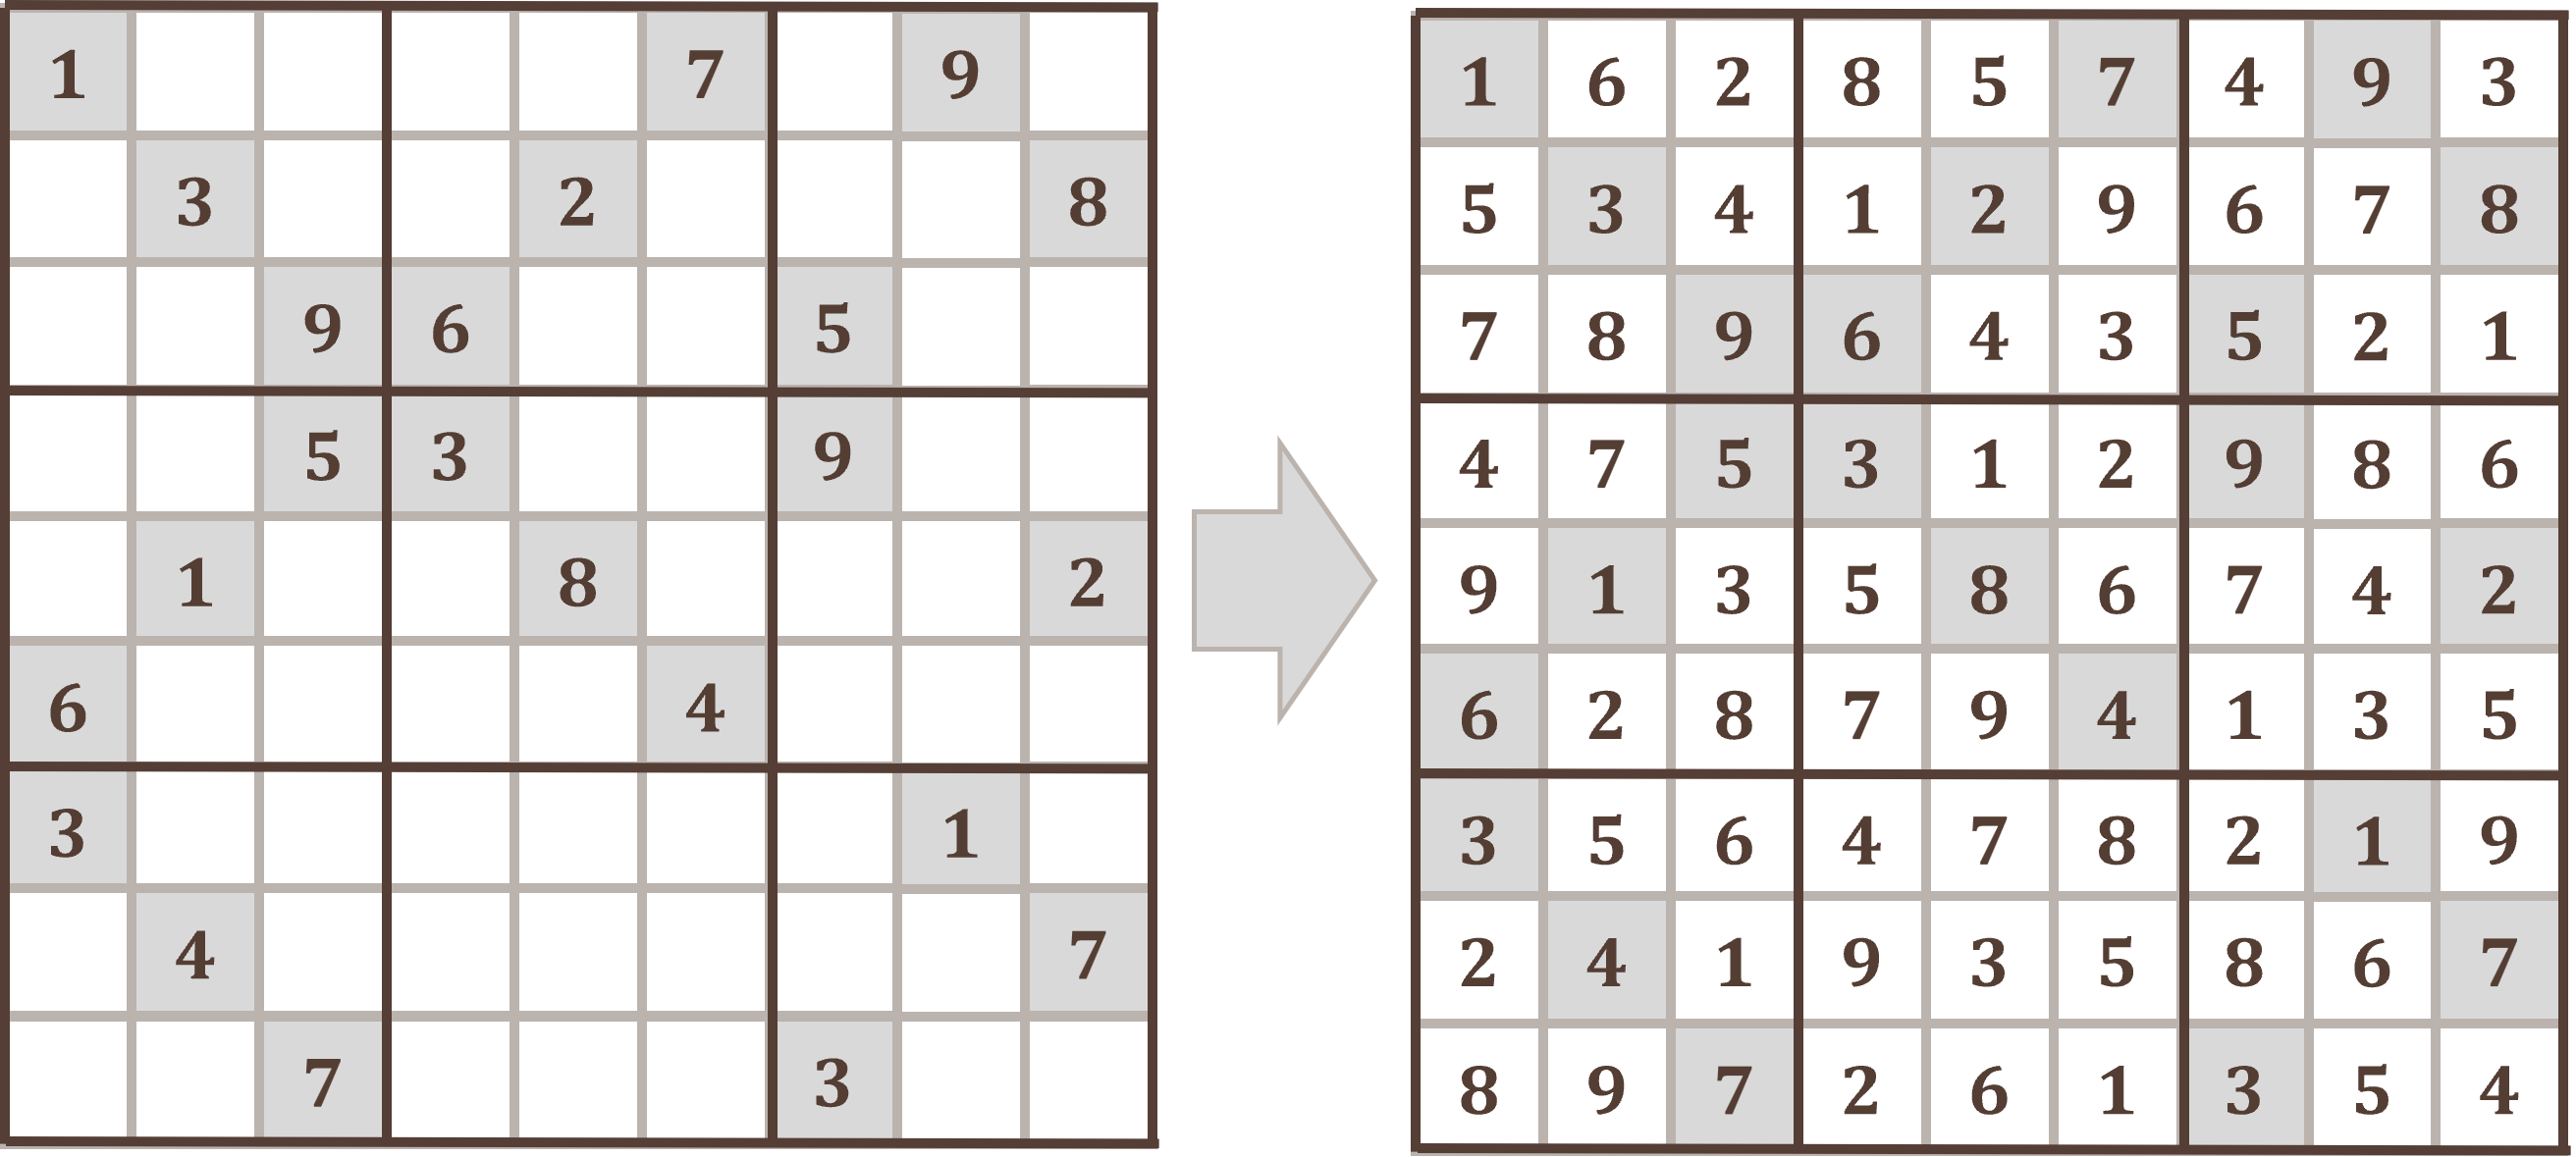
\includegraphics[width=\columnwidth]{Img/Sudoku.png}
%     \bicaption {名为“AI Escargot”的数独实例。} {A Sudoku instance called "AI Escargot".}
%     \label{fig:Sudoku}
% \end{figure*}

% \section{本章小结}
% 在这一章中,介绍了算法的补充策略,解池技术及其维护。具体地,
% 在第一节中,本文介绍了解池技术的基本概念,以及分别通过解近似和扰动策略构造的解的准入和生成策略。
% 在第二节中,本文介绍了基于解池技术的加权和动态迭代策略,具体地,算法构造了新的WACG,并根据求解情况动态地调整后续求解的迭代次数。
% 在第三节中,本文通过构造新的冲突类型,将二元约束引入到求解的框架中,并介绍了实现的求解工具的具体细节。